Next up, the joint IAAI/AAAI talk on smart cities.

\subsection{Invited Talk: Yu Zheng on Smart Urban Cities}

Consider: Rapid Progress of urbanization. Has led to huge challenges in dense urban areas, from traffic to housing. \\

{\bf Vision:} Use urban computing to improve lives in cities through:
\begin{itemize}
    \item Urban Sensing
    \item Data Management
    \item Data Analytics
    \item 
\end{itemize}

\begin{figure}[h!]
    \centering
    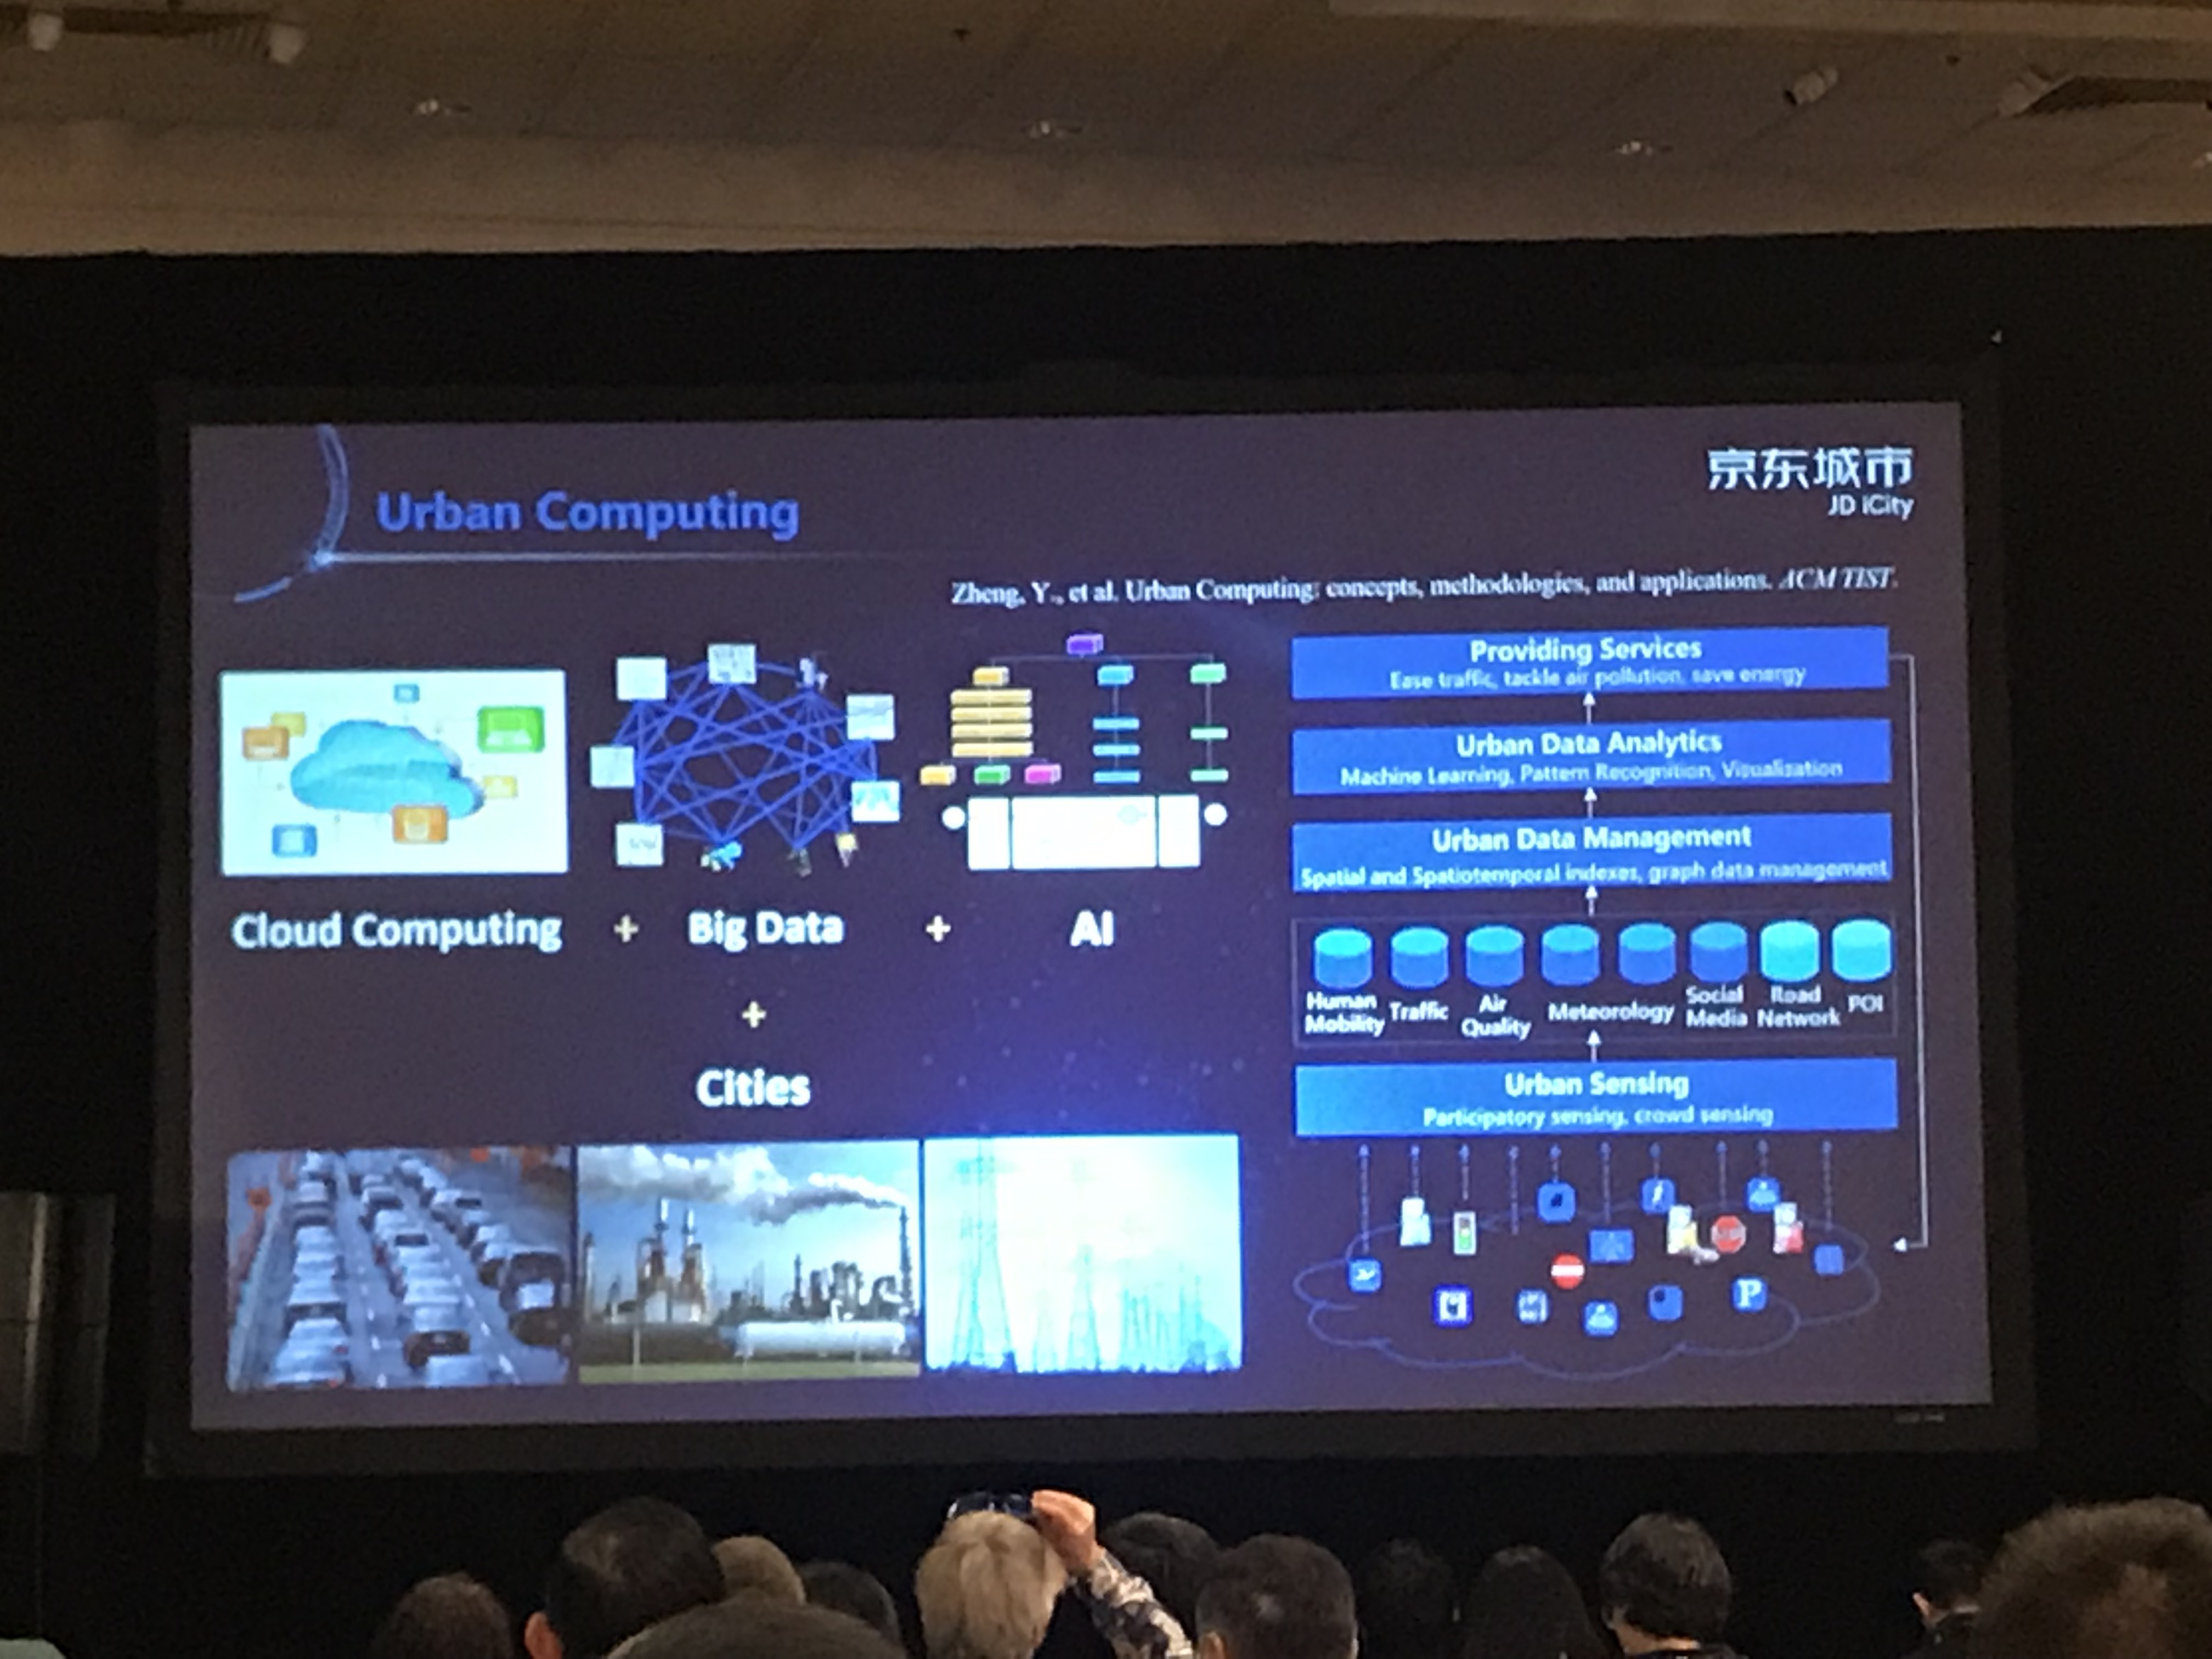
\includegraphics[width=0.5\textwidth]{images/urban.JPG}
    \caption{Overview of urban computing vision.}
    \label{fig:urban}
\end{figure}



\subsubsection{Challenge 1: Urban Sensing}

Challenges:
\begin{enumerate}
    \item {\it Resource deployment:} How should we deploy sensors to gather the right data? Candidate selection is an NP-Hard problem.
    \item {\it Measuring:} Hard to define a measurement for evaluating the deployment
    \item {\it Biased samples:} taxi flow vs. traffic flow. Taxi traffic is biased toward particular routes (but we can get taxi data).
    \item {\it Data Sparsity:} limited air quality sensors but want fine grained air quality throughout a city.
    \item {\it Data Missing:} Communication/sensor errors.
\end{enumerate}

If we can overcome these challenges, we can then collect a diversity of data: air quality, pedestrian traffic, bus use, etc. \\

$\ra$ Summarize data into a particular 6 kind ontology, based on their spatio-temporal type (static, temporal, dynamic, and point-based vs. network based. Goal is to make this scalable so that any new data types can be captured into the future. Summarized in Figure~\ref{fig:data_type}.

\begin{figure}[h!]
    \centering
    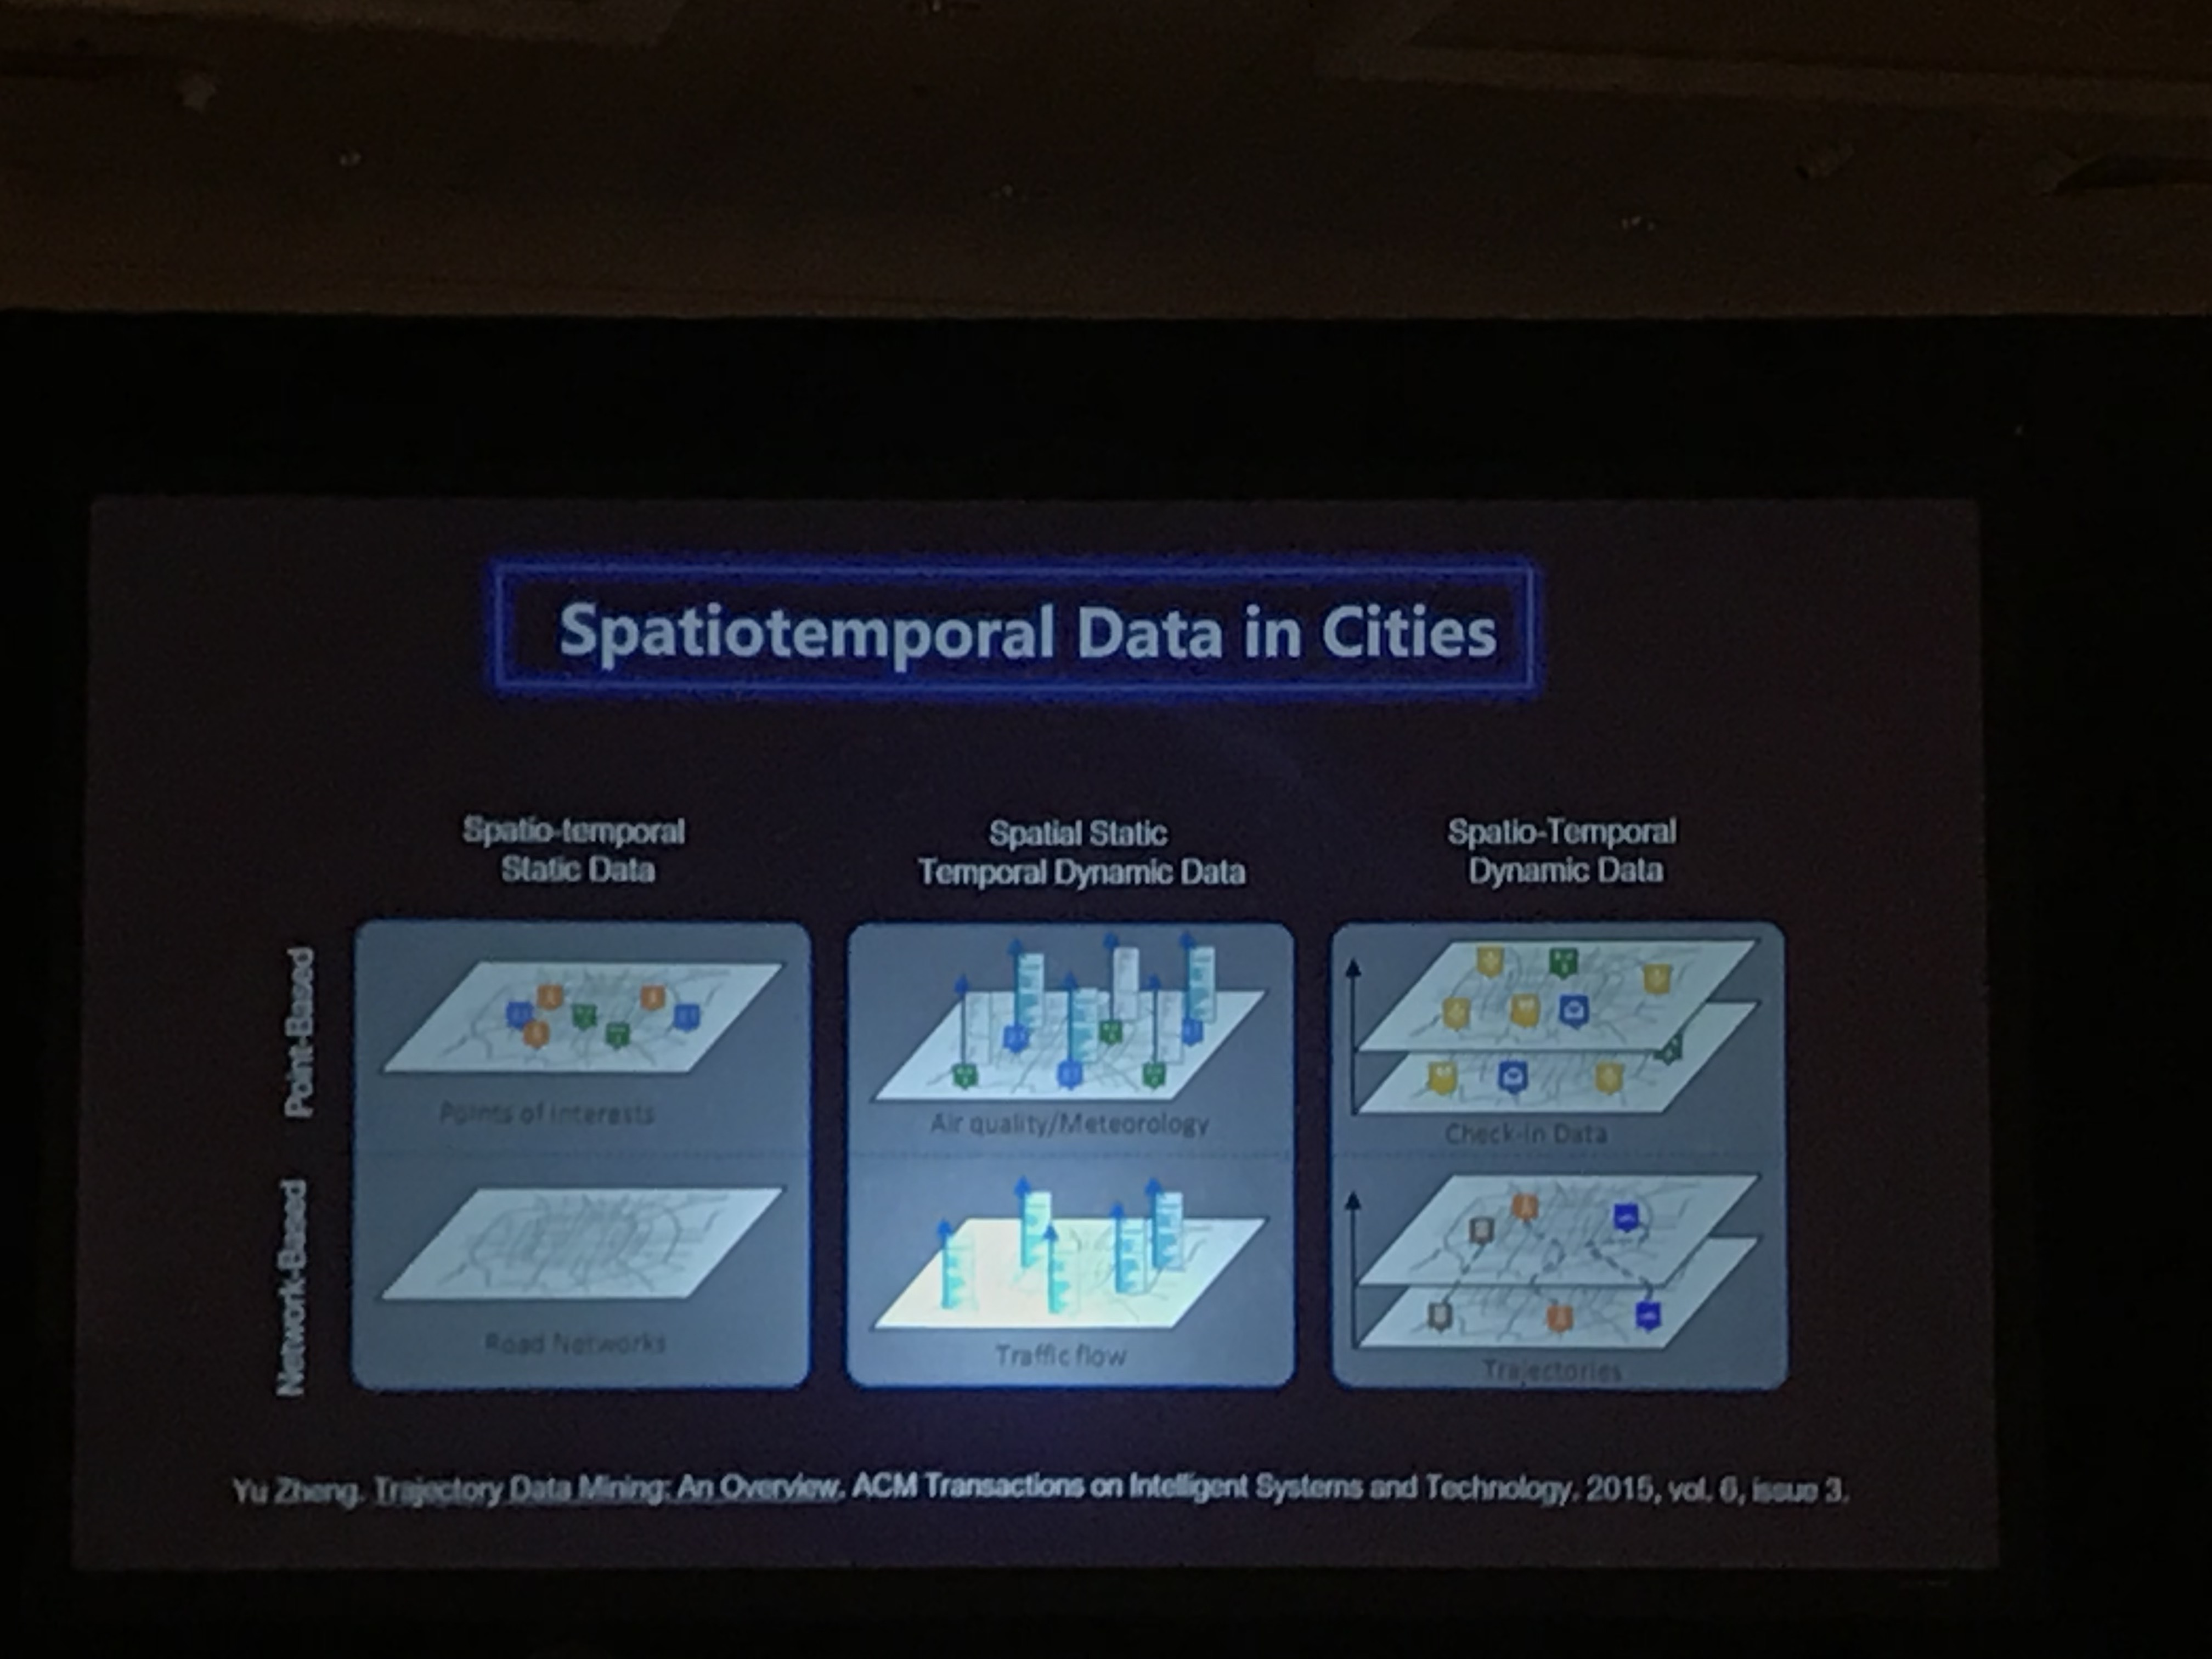
\includegraphics[width=0.5\textwidth]{images/data_type.JPG}
    \caption{Categorization of kinds of data in urban computing, designed to scale with new types of cities/data/challenges.}
    \label{fig:data_type}
\end{figure}

Spatiotemporal data is unique:
\begin{itemize}
    \item Spatial properties like distance, correlation. We can even apply triangle inequality.
    \item Spatial hierarchy: different spatial/geographic granularities, such as buildings $\in$ neighborhoods $\in$ districts.
    \vspace{2mm}
    \item Temrporal closeness, period, and trend give us further structure to exploit.
\end{itemize}

\subsubsection{Challenge 2: Data Management}

{\bf Problem:} large scale (city level!). So we need to handle a huge volume of data efficiently. \\

Hard to handle spatiotemporal data in particular:
\begin{itemize}
    \item Trajectory data is represented by a sequence of data types is highly complex.
    \item Unique queries make searching the data difficult.
    \item Data is spread across different domains, so requires hybrid indexing for maning multi-modal data.
\end{itemize}

Example: detect vehicle illegal parking using bike-share trajectories. \\

$\ra$ Solution: Can spot when bikes take odd swerves on a road to estimate where cars might be parked illegally~\cite{he2018detecting}. Use classification to spot the anomalous trajectories. \\


\subsubsection{Challenge 3: Data Analytics}

Example: Predicting crowd flows in a city. Difficult because of complex factors that effect this situation -- depends on time, events, weather, traffic, and so on. \\

$\ra$ Solution: partition a city into a uniform grid. Count the in flow and outflow of people in each grid cell over time. Now, given this series of grid-based-heat-maps, want to predict the grid at the next time-frame. Most off the shelf deep learning models don't capture the relevant spatio-temporal structure. Instead, develop a new architecture that looks for specific structure relevant to the domain~\cite{zhang2017deep}. \\

%\subsubsection{Mining Data from Different Domains}

{\bf Problem:} Air pollution is a global concern. Monitoring air quality is extremely difficult. \\

Solution: infer real-time and fine-grained air quality through a city~\cite{zheng2013u}. Provide a user interface for zooming in and out of a city to check the air quality at different regions of a city. Can even identify the source of solution. \\

$\ra$ Deployed in over 300 cities in china(!). Even offers prediction over the next 48 hours--\\

\subsubsection{Challenge 4: Providing Services}

Developed: urban computing platform that can accommodate the 6 types of data discussed previously, specially tuned for spatiotemporal data. \\

Opens up the opportunity for cities to share data and tools to improve inference and analytics. \\

Deployed: JD iCity, can play with it here: \url{http://ucp.jd.com} (\dnote{just a heads up it's in chinese}).

Summary:
\begin{itemize}
    \item Framework for urban computing
    \item Many research challenges, some effective solutions so far
    \item Urban computing platform as an OS for cities.
\end{itemize}

\spacerule

\subsection{Reasoning Under Uncertainty}

Now for some reasoning under uncertainty.


\subsubsection{On Testing of Uniform Samplers~\cite{chakraborty2019testing}}

Paper by Sourav Chakraborty and Kuldeep Meep. \\

Andrew Ng: ``AI is the new electricity" \\

And yet, it fails basic tasks: ``Im a huge metal fan" $\ra$ (translate to french) ``I'm a large ventilated object." \\

{\bf This Work:} Verification. \\

Given a model $M$, like a neural network to label images, and a specification, $\varphi$, that specifies the goals of $M$. \\

Idea of verification: We can check whether there exists an execution of $M$ that violates $\varphi$.\\

Q: Yes, but so what? \\

A: Well, samplers form the core of the state of the art probabilistic reasoning techniques. Can use Markov Chain Monte Carlo (MCMC). Use statistical test to argue for quality of the sampling distribution. \\

Example: suppose we're uniformly sampling from a domain from 1 to $N$. Distance is total variation distance ($\ell_1$). How many samples do we need before getting a collision?\\

\begin{theorem}
Testing whether a distribution is $\eps$-close to uniform has query complexity $\Theta(\sqrt{S}/\eps^2)$, with $S$ the size of the domain(?) \dnote{missed citation -- from another paper}.
\end{theorem}

\ddef{Conditional Sampling}{Given a distribution $D$ on domain $S$, one can specify:
\begin{itemize}
    \item Specify a set $T \subset D$
    \item Draw samples according to the distr. $D_T$, that is, $D$ under the condition that the samples belong to $T$.
\end{itemize}}

Clearly, such a sampling technique is {\it as powerful} by setting $T$ to the full support. But, what else can we do? \\

Sampling algorithm (for the two ``true" uniform and non-uniform case -- how can we determine which distr we are sampling from?):
\begin{itemize}
    \item Pick two elements uniformly at random $x,y$.
    \item In the case of the ``far" distribution, one of the elements will have Pr $0$, and the other $\Pr > 0$.
    \item Now a constant number of conditional samples is enough to identify that the distribution is not uniform.
\end{itemize}


Q: What about other distributions? \\

A: Need a few more tests, but largely same idea as the above. \\

Consider: uniform sampler for CNF formulas: Given a CNF formula $\phi$ and a CNF sampler $A$, that outputs a random solution of $\phi$.

\ddef{CNF Sampler}{A CNF-Sampler $A$ is a randomized algorithm that, given a $\phi$, outputs a random element of the set $S$, such that for any$x\in S$:
    \[
    Pr(A(\phi) = x) = \frac{1}{|S|}
    \]
}

Main problem: come up with a good CNF sampler. \\

Algorithm: Similar idea to before, yields the following main result:
\begin{theorem}
Given $\eps, \eta, \delta$, the number of samples the above their algorithm needs to accept/reject the formula,
\[
K = \tilde{O}\left(\frac{1}{(n-\eps)^4}\right),
\]
samples for any input formula $\phi$.
\end{theorem}

Experiments: compare different CNF sampling algorithms on a variety of benchmarks. \\

Conclusion:
\begin{itemize}
    \item Need methodological approach for verification of AI systems.
    \item Need to go beyond qualitative verification to probabilistic verification.
    \item Sampling is a crucial component of the state of the art probabilistic reasoning systems.
    \item This work: property testing meets verification, promise strong theoretical guarantees.
\end{itemize}




\spacerule
\subsubsection{Finding All Bayes Net Structures Near-Optimally~\cite{liao2018finding}}

Paper by Zhenyu Liao, Charupriya Sharma, James Cussens, and Peter van Beek. \\

\ddef{Bayes Nets}{A directed acyclic graph (DAG) that model a joint distribution over a set of random variables}

Bayes Nets can model conditional independence and causation, they can learn and model structure in data. \\

Structure Learning: learn a Bayes Net from data using a score-and-search approach, given training data of $N$ instances. \\

$\ra$ Lots of approaches to structure learning -- 1) consider space of all DAGs, 2) restrict your structure, or 3) consider only the best $k$-scoring DAGs.\\

Problem: restricting structure too much might limit the Bayes Net, if you don't limit it won't scale. \\

{\bf This Work:} Structure learning that fixes both of the above problems. \\

Main Results:
\begin{itemize}
    \item Propose a novel approach to model averaging inspired by approximation algorithms
    \item Approach only consider models that are optimal or near-optimal (in score).
    \item Prove this approach is efficient and can scale to much larger networks than the SOTA.
\end{itemize}

\ddef{$\eps$-BNSL}{Given $\eps > 0$, a dataset $I$ over variables $V$ and a scoring function $\sigma$, the $\eps$-Bayes Net Structure Learning (BNSL) problem finds all networks:
\[
OPT \leq score(G) \leq OPT + \eps,
\]
where $\eps = (\rho-1) OPT$.}

Problem closely related to Bayes Factor (BF), which can be interpreted as a measure for the relative success of a model to predict data. \\

Other problem: scaling. \\

$\ra$ Solution: prune the search space --
\begin{theorem}
(From~\citet{teyssier2012ordering}) Given a vertex and two parent sets $\Pi$ and $\Pi'$, we can prune the if $\Pi \subset \Pi'$ and $\sigma(\Pi) \leq \sigma(\Pi')$, then $\Pi'$ can be safely pruned.
\end{theorem}

This work extends this theorem to the $\eps$-optimal case:
\begin{theorem}
Given a vertex and two parent sets $\Pi$ and $\Pi'$ and $\eps \geq 0$, we can prune the if $\Pi \subset \Pi'$ and $\sigma(\Pi) + \eps \leq \sigma(\Pi')$, then $\Pi'$ can be safely pruned.
\end{theorem}

Experiments show that their approach both scales and achieves near-optimal scores.

\spacerule
\subsubsection{Rethinking the Discount Factor in RL~\cite{pitis2019rethinking}}

Paper by Silviu Pitis. \\

Original title: ``The MDP is all you need!" -- we think that MDPs can sufficiently account for all the modeling power that we need. \\

Set out to show that MDPs are sufficient for general intelligence by defining some axioms and deriving rational behavior in MDPs. But, I couldn't do it. So, instead I'll be talking about rethinking the discount factor. \\

Why like the MDP as a model?
\begin{itemize}
    \item Preferences induced by the discounted value function satisfy several notions of consistency (our axioms!)
    \item Fundamental theorem of Inverse RL -- any abirtrary behavior can be represented as the optimal policy in some MDP~\cite{ng2000algorithms}.
\end{itemize}

Q: So, why might the MDP fail to model preferences? \\

A1: Human preferences are complex -- maybe agent can't learn the ``optimal policy". \\

A2: We have good reason to model preferences with respect to suboptimal policies. \\

A3: Cliff example in this paper gives a numerical example of the above. \\

MDPs can't model {\it arbitrary} preferences. Let $A$ and $B$ be two events. Then:
\begin{align}
    ABAAAA > AAABAAAA  > AABAAAA,
\end{align}
can't be captured. But, it's irrational to do that anyway.\\

$\ra$ What we care about is capturing {\it rational} behavior. \\

\ddef{Rationality}{Characterized by axioms that we agree preferences should satisfy, as in the Von Neuman and Morgenstern axioms (Completeness, Transitivity, Independence, Continuity, and some time-axioms Irrelevance, Dynamic Consistency, and Impatience)}

This work: define rational preferences over actions, states, and policies. MDPs induce preferences according to:
\[
\text{if  } V^1(s_1) > V^2(s_2)\hspace{6mm} \text{then } (s_1, \pi_1) > (s_2, \pi_2)
\]

Main result:
\begin{theorem}
There exist $\mc{R} : S \times A \ra \mathbb{R}$ and $\Gamma: S \times A \ra \mathbb{R}^+$ such that for all $s,a,\pi$:
\begin{equation}
    U(s,a,\pi) = R(s,a) + \Gamma(s,a) \bE_{s'\sim T(s,a)}[U(s', \Pi)].
\end{equation}
\end{theorem}
Closest thing to the usual rationally result -- basically, we need to think about discount factor as a function of $(s,a)$ instead of being fixed. \\

Q: Given the observed behavior, what utility function (parameterized by both reward and discount), is being optimized? \\

A: Nice direction for future work!

\spacerule

\subsection{Invited Talk: Tuomas Sandholm on Solving Imperfect Information Games}

Note: most real-world applications are imperfect information games. \\

Recently achieved superhuman AI performance in imperfect information games. \\

Q: How do we do it? \\

A: Techniques for perfect information games won't work. But, can rely on application/task specific techniques! \\

{\bf Challenges:} 1) Uncertainty about what others and chance will do, 2) Hidden state, so we need to interpret signals and {\it use game theory}. \\

$\ra$ The game theory is critical! But, hard to scale computationally. So, major challenge is scaling the game theory. \\

Libratus overview pictured in Figure~\ref{fig:libratus}. \\

\begin{figure}[h!]
    \centering
    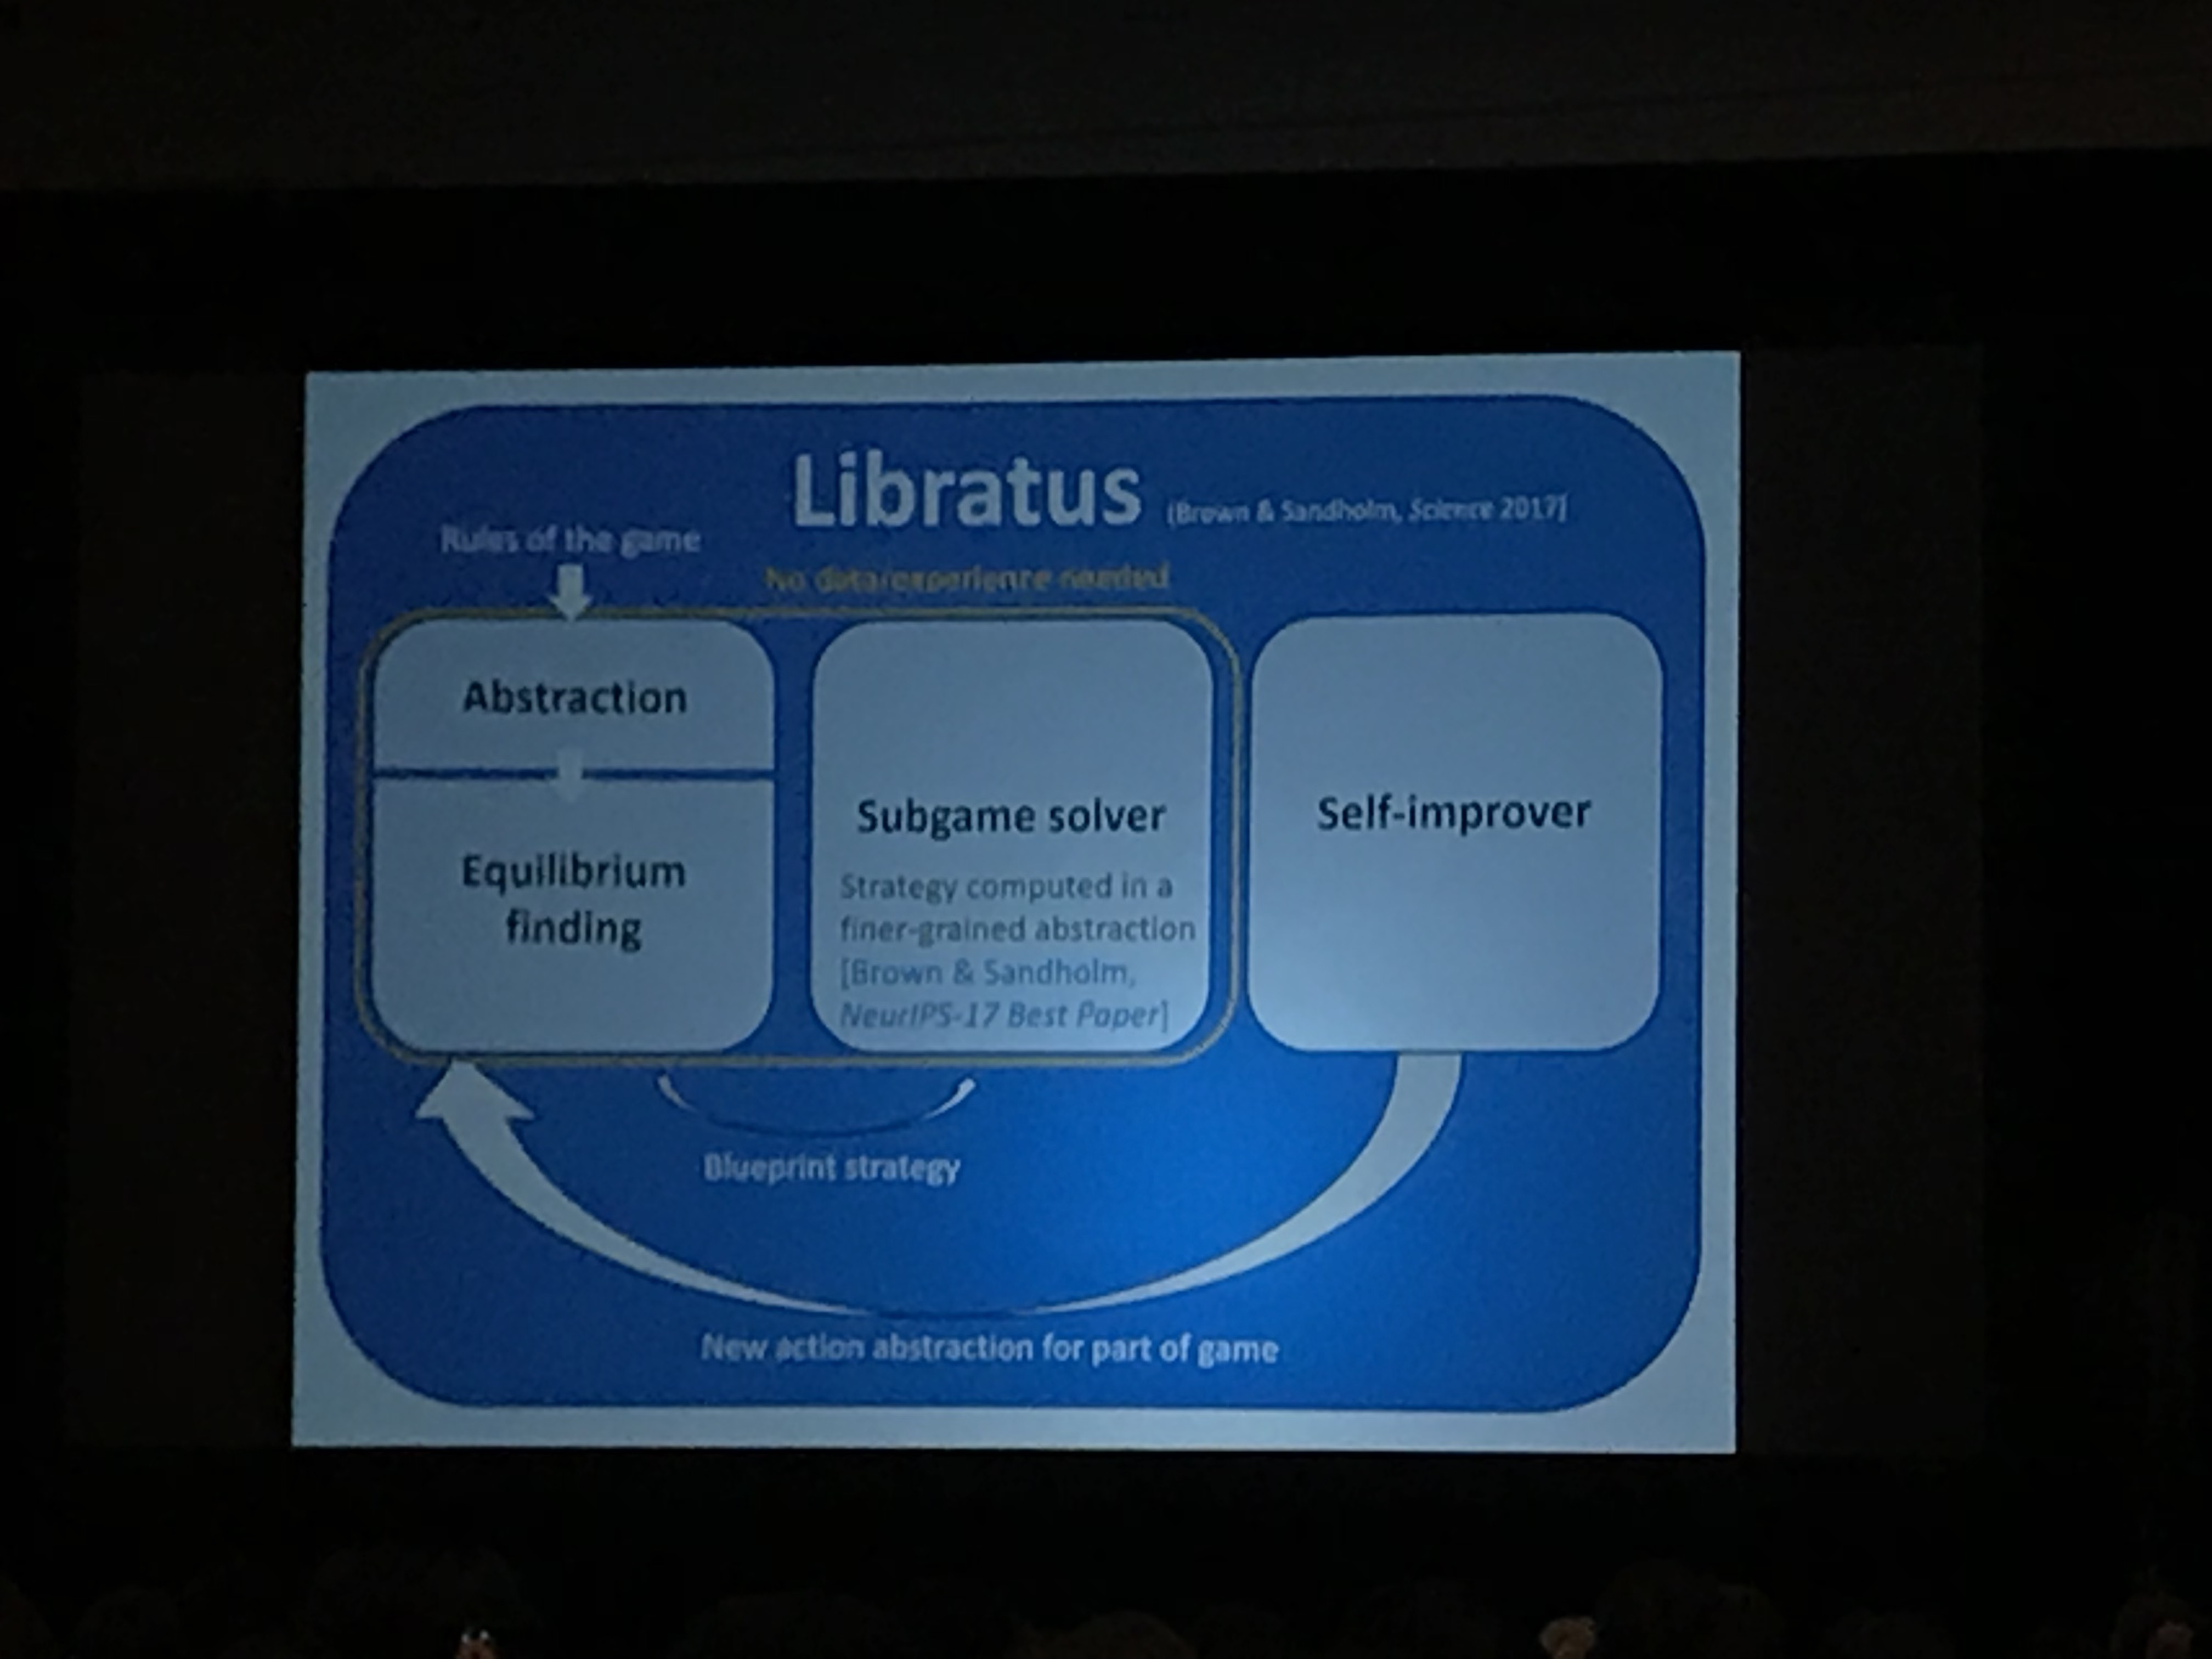
\includegraphics[width=0.5\textwidth]{images/libratus.JPG}
    \caption{Overview of Libratus.}
    \label{fig:libratus}
\end{figure}

\ddef{Extensive Form Game (EFG)}{Game with some chance and $N$ players is an extensive form game. Also defines a game tree of possibilities over plays, with payoff at the leaves (general sum).}

Strategies for EFG: behavioral strategy $\sigma_i$ with $i$ an information set. Specifies a distribution over actions. \\

Player $i$'s utility of strategy profile ($\sigma_1, \sigma_2)$. \\

$\eps$-Nash Equilibrium: strategy profile such that no player can improve behavior by more than $\eps$ by changing strategy. \\

Talk Roadmap:
\begin{itemize}
    \item Abstraction: unifed framework for game abstraction with solution quality bounds.
    \item Finding Nash Equilibrium: fast algorithms for solving games.
    \item Equilibrium Refinement
\end{itemize}

\subsubection{Abstraction}

Started with lossless absstraction~\cite{gilpin2007lossless} but, found we needed to move to lossy abstraction. Turns out abstraction in games in non-monotonic~\cite{waugh2009abstraction} \\

Q: Can we get bounds on solution quality anyway?  \\

A: Yes!~\cite{sandholm2012lossy}. Also applies to abstraction, since modeling is just abstraction. \\

Abstraction theorem:
\begin{theorem}
Given a perfect-recall game, an acylic abstract game, a mapping between the two games that satisfies mild assumptions, an $\eps$-Nash equilibrium in the abstract game, then: any lifted strategy is an $\eps$-Nash equilibrium in the original game:
\[
\eps' = \eps + \text{ mapping error } + \text{ refinement error.}
\]
\end{theorem}

Rest of the talk: theorems apply to 2-player, 0-sum games, but they're intended to apply to more general games. \\

Counterfactual regret minimization (CFR): used by every top poker AI in the past 5 years. Used a tabular form of CFR and abstraction before equilibrium finding. \\

$\ra$ Next up they introduce a function approximator for use in CFR (leads to ``Deep CFR"). \\

Chicken-and-egg problem with abstractions: hard to pick an abstraction without knowing the equilibria, but hard to find the equilbiria without using an abstraction. \\

$\ra$ Solution: do both simultaneously! \\

Monto Carlo CFR~\cite{lanctot2009monte}:
\begin{itemize}
    \item Action regret is how much better we would have done had we always picked this action in this situation in the past.
    \item Do Monte Carlo roll outs, always pick action proportional to {\it positive regret}.
\end{itemize}

\subsubection{Finding Nash Equilibria}

{\bf Motivation:} Previous fastest solver is CFR+, but has some sever limitations (namely: requires a huge number of iterations to pick the right action early ). \\

$\ra$ Gives rise to linear CFR, which is a dramatically more efficient method than CFR (from 500,000 iterations to around a few hundred). \\

Two ideas:
\begin{enumerate}
    \item Linear CFR: Weight iteration by recency for efficiency gains
    \item CFR+: floor regrets at zero
\end{enumerate}

Q: Can we combine them? \\

A: Theory $\ra$ yes! Practice $\ra$ no. \\

But, less aggressive combinations do well. This yields discounted CFR, which combines good aspects of each of these things. \\

Conducted experiments in Heads-Up No-Limit Texas hold'em (henceforth "texas") $\ra$ DCFR and LCFR both dominate nearly all other strategies. \\

Q: What about Monte-Carlo variants? \\

A: Doesn't mix well with DCFR, but does mix with linear CFR quite well. \\

{\bf Limitations of CFR:}
\begin{itemize}
    \item Usually for 2 player games
    \item Only works with linear loss
    \item Doesn't support behavioral constraints
\end{itemize}
Next up: they'll fix all three of these. \\

Consider the ``sequential decision making" strategy space~\cite{farina2018online}. \\

Idea: define a local notion of regret $\hat{R}$ at each decision point of the player.

\begin{theorem}
We can get an extension of the usual result of CFR but for any convex loss function (not just linear) based on the local regret:
\[
R^T = \ldots \leq \max_x \sum_{j \in J} \pi_j(x) \hat{R}_j^T
\]
\end{theorem}

This new framework is much more general and can be applied to a variety of new applications. \\

{\bf Hot Off the Press:}
\begin{itemize}
    \item {\it Regret Circuits:} compositional calculus of regret minimizers.
    
    $\ra$ Can support strategy constraints that cut across ``infoset"s.
    
    \item {\it Breaking the complexity barrier:} new decomposition yields a CFR-like algorithm but converges in $O\left(\frac{1}{T^{\frac{3}{4}}}\right)$ instead of $O\left(\frac{1}{T^{\frac{1}{2}}}\right)$. First ever CFR like algorithm to break this barrier!
\end{itemize}

Perfect information games and single agent search: take some steps, then solve remaining subtree. If tree is too big, we break off a small chunk, and try to solve that subset. \\

Idea: depth-limited solving (DLS)~\cite{brown2018depth}. In Libratus, when we solve a game, we solve it {\it all the way to the end of the game.} In things like ``deep stack" they do this depth limited solving, but in an expensive way (random subgames solved in advance). \\

$\ra$ New Approach for solving DLS:
\begin{itemize}
    \item At the leaf nodes at the depth limited tree, we allow the other player $P_1$ to choose a continuation policy.
    \item Solve the subgame with the current set of continuation policies
    \item Calculate best response for $P_2$.
    \item Add best response to set of leaf-node policies.
\end{itemize}
\dnote{Not sure I got the player numbers right in the above..}

\begin{theorem}
The above approach converges to Nash equilibrium.
\end{theorem}

Moreover, the above reaches very low exploitibility in a small number of iterations. \\

{\bf Key Takeaways:}
\begin{itemize}
    \item Planning is important in imperfect information gatmes
    \item In real time planning you must consider how the oppeonent can adapt to changes in your policy
    \item States don't have well defined values in imperfect info games
    \item New bot developed end-to-end on a single computer is 2nd best AI bot after Libratrus.
\end{itemize}

\subsubsection{Equilibrium Refinement}

{\bf Major Point:} An issue with Nash: assumes strongest possible opponent! So, it doesn't capitalize on opponents' mistakes. \\

$\ra$ Enter, refinements, which can help to improve. \\

Idea: Mandate that users play each action at each information set. This enables reasonable strategies and beliefs to be computed even in non-standard parts of the game tree. Enables refinement!\\

Can formulate this problem as a Linear Program (LP), parameterized by $\eps > 0$. Theory says there is an $\eps^* \in \mathbb{R}_{\geq}$ such that the LP can be computed in polynomial time and achieve good performance (finding a good ``basis"). \\

But, the above induces an unusably slow algorithm for refinement (that has desirable properties). Instead, don't look for $\eps^*$, look at something a bit weaker $\ra$ gives rise to a practical algorithm. \\

Bottom line: refinements of Nash Eq matter when some players are not fully rational. \\

Consider Stackelberg games: extensive form games {\it with commitment}.
\begin{itemize}
    \item One player commits to a public mixed strategy (``leader")
    \item Another play (``follower")
\end{itemize}

Goal is another equilibrium: ``strong" stackelberg equilibrium) assume follower breaks ties in best possible way for leader). \\

$\ra$ Same issue as Nash: assumes fully rational opponent. \\

Q: Is trembling-hand perfection meaningful in Stackelberg games? \\

A:
\begin{theorem}
\begin{itemize}
    \item Trembling-hand Stackelberg equilibrium are Stackelberg equilibrium
    \item Finding a Stackelberg equilibrium is NP-Hard
    \item Finding a $\tau$-Stackelberg equilibrium is NP-Hard.
\end{itemize}
\end{theorem}

{\bf Conclusion:}
\begin{enumerate}
    \item Imperfect info games are important but different
    \item Game-theoretic techniques are required to be robust against all opponents
    \item Modern techniques for these ($=$imperfect info games) should be taught in AI courses
    \item Talked about abstraction and its role in CFR
    \item Finding Nash equilibria can be done scalably
    \item May want to refine equilibria sometimes.
\end{enumerate}

Future Work:
\begin{itemize}
    \item Merge practical abstraction algorithm with new abstraction theory
    \item Even bigger games! Deeper/infinite, large branching factors
    \item Techniques that work with blackbox access to the world
\end{itemize}

And that's Thursday! Now onto the poster session.

\spacerule
